\documentclass[pdf]{beamer}

\usepackage{rsislidepacks}
\usepackage{colortbl}
\usepackage{enumerate}
\usepackage{hyperref}
\usepackage{asymptote}
\usetheme{UNLTheme}
\setbeamercovered{dynamic}

\usepackage{tikz}
\usetikzlibrary{shapes,arrows}

\def\ii{\item}
\def\ul#1{\underline{#1}}
\def\AA{\mathcal A}
\def\MM{\mathcal M}
\def\RR{\mathbb R}
\def\ZZ{\mathbb Z}
\def\half{\frac{1}{2}}
\newcommand{\defeq}{\stackrel{\text{def}}{=}}
\newcommand{\dobarbell}[2]{
\vcenter{\hbox{%
\includegraphics[scale=#1]{barbell/#2.pdf}
}}
}
\newcommand{\barbell}[1]{
\mathchoice%
{\dobarbell{1.6}{#1}}
{\dobarbell{1.2}{#1}}
{\dobarbell{0.9}{#1}}
{\dobarbell{0.9}{#1}}
}
\def\stimes{\otimes_{R^s}}
\def\ttimes{\otimes_{R^t}}


\begin{asydef}
	import olympiad;
	import cse5;
	pointpen = black;
	pathpen = black;
	pathfontpen = black;
	anglepen = black;
	anglefontpen = black;

	pen s = blue, t = red;
	pen dot_s = blue, dot_t = red;
\end{asydef}

\begin{document}
\title[Bott-Samelson Bimodules]{Diagrammatic Computation of Morphisms Between Bott-Samelson Bimodules via Libedinsky's Light Leaves}
\subtitle[RSI 2013]{Research Science Institute 2013}
\author[Evan Chen]{Evan Chen \\ Under the Direction of Francisco Unda, MIT Math \\ Project Provided by Ben Elias, MIT Math\vspace{-2em}}
\date{August 1, 2013}

\begin{frame}
	\maketitle
\end{frame}

\section{Background}
\begin{frame}[fragile]
	\frametitle{Background}
	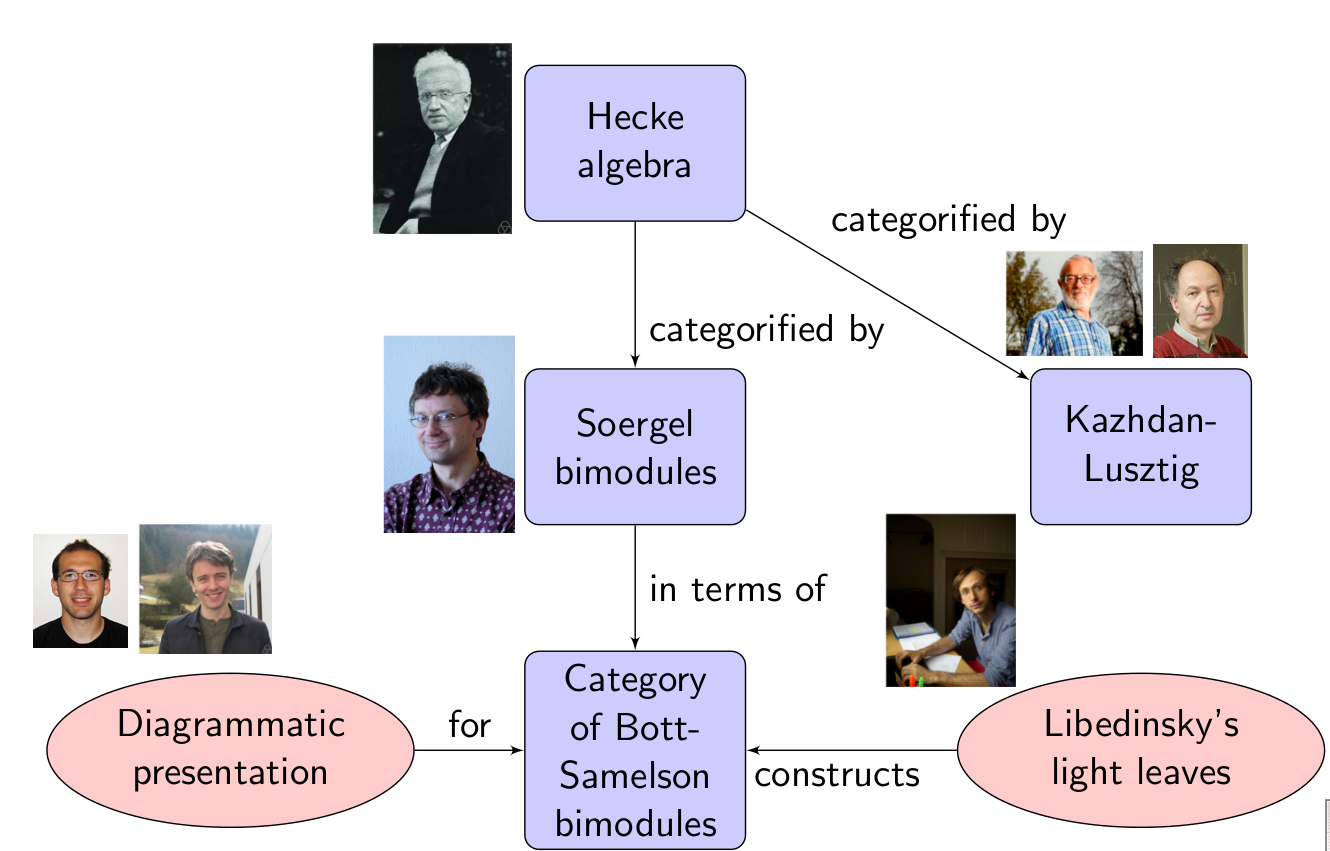
\includegraphics[width=0.95\textwidth]{hecke.png}
	% Define block styles
%	\tikzstyle{block} = [rectangle, draw, fill=blue!20, text width=5em, text centered, rounded corners, minimum height=4em]
%	\tikzstyle{cloud} = [draw, ellipse,fill=red!20, node distance=3cm, text width=6em, text centered, minimum height=2em]
%	\tikzstyle{line} = [draw, -latex']
%	\scalebox{0.8}{
%	\begin{tikzpicture}[node distance = 4cm, auto]
%		% Place nodes
%		\node [block] (Hecke) at (0,6) {Hecke algebra};
%		\node [block] (Soergel) at (0,3) {Soergel bimodules};
%		\node [block] (KL) at (5,3) {Kazhdan-Lusztig};
%		\node [block] (BS) at (0,0) {Category of Bott-Samelson bimodules};
%		\node [cloud] (leaf) at (5,0) {Libedinsky's light leaves};
%		\node [cloud] (diag) at (-4,0) {Diagrammatic presentation};
%		% Draw edges
%		\path [line] (Hecke) -- node [near end] {categorified by} (Soergel);
%		\path [line] (Hecke) -- node [near start] {categorified by} (KL);
%		\path [line] (Soergel) -- node {in terms of} (BS);
%		\path [line] (leaf) -- node [text width=5em] {constructs} (BS);
%		\path [line] (diag) -- node {for} (BS);
%	\end{tikzpicture}
%	}
\end{frame}

\section{Prerequisites}
\begin{frame}[fragile]
	\frametitle{Diagrammatics}
	\begin{itemize}
		\ii Diagrams are drawn with top/bottom boundary.
		\ii The maps are represented as red/blue planar graphs.
		\ii Vertices have degree $1$ or $3$.
		\ii Isotropy invariant: 
		\begin{asy}
			size(9mm,4mm);
			draw((-2,-3)--(-2,2), t);
			draw((0,0)..(1,1)..(3,0)..(2,-2)..(5,0), s);
			dot((-2,-3), dot_t);
			dot((-2,2), dot_t);
			dot((0,0), dot_s);
			dot((5,0), dot_s);
		\end{asy}
		\ is the same as
		\begin{asy}
			size(9mm,4mm);
			draw((-1,-1)--(-1,1), s);
			draw((0,-1)--(0,1), t);
			dot((-1,-1), dot_s);
			dot((-1,1), dot_s);
			dot((0,-1), dot_t);
			dot((0,1), dot_t);
		\end{asy}
		.
	\end{itemize}
	\begin{figure}[ht]
		\centering
		\begin{asy}
		size(4cm);
		real xmax=7;
		real ymax=5;
		draw((xmax,ymax)--(-xmax,ymax));
		draw((xmax,-ymax)--(-xmax,-ymax));
		draw((xmax,-ymax)--(xmax,ymax), dotted);
		draw((-xmax,-ymax)--(-xmax,ymax), dotted);
		pair apex = (0,2);
		path arc = (5,-5)..(2,0)..apex..(-2,0)..(-5,-5);
		draw(arc, s);
		dot(apex, dot_s);
		draw(apex--(0,ymax), s);
		draw(-apex--(0,-ymax), t);
		dot(-apex, dot_t);
		label("$s$", (0,ymax), dir(90));
		label("$t$", (0,-ymax), dir(270));
		label("$s$", (-5,-ymax), dir(270));
		label("$s$", (5,-ymax), dir(270));
		\end{asy}
		\begin{asy}
		size(4cm);
		real xmax=7;
		real ymax=5;
		draw((xmax,ymax)--(-xmax,ymax));
		draw((xmax,-ymax)--(-xmax,-ymax));
		draw((xmax,-ymax)--(xmax,ymax), dotted);
		draw((-xmax,-ymax)--(-xmax,ymax), dotted);
		draw(CR((2,0),3), t);
		draw(Drawing((2,-3),dot_t)--(2,-ymax), t);
		draw(Drawing((3,0),dot_s)--Drawing((1,0),dot_s), s);
		draw(Drawing((-6,-1),dot_t)--Drawing((-6,1),dot_t), t);
		draw(Drawing((-4,-1),dot_s)..(-3,2)..Drawing((-2,-1),dot_s), s);
		// draw(Drawing((5,ymax-1.414),dot_s)..(5,ymax),s);
		label("$s$", (5,ymax), dir(90), white);
		label("$t$", (2,-ymax), dir(270));
		\end{asy}
		\caption{Examples of diagrams.}
		\label{fig:example_diagram}
	\end{figure}
\end{frame}

\begin{frame}
	\frametitle{Libedinsky's Light Leaves}
	\begin{itemize}
		\ii Start with string $\ul r$ (letters $s$ and $t$) and a binary string $\ul b$.
		\ii Read the bits from left to right.
	\end{itemize}
	\begin{figure}
		\centering
		%\aoeu{1}\aoeu{2}\aoeu{3}\aoeu{4}\aoeu{5}\aoeu{6}\aoeu{7}\aoeu{8}\aoeu{9}\aoeu{10}\aoeu{11}
		\only<1>{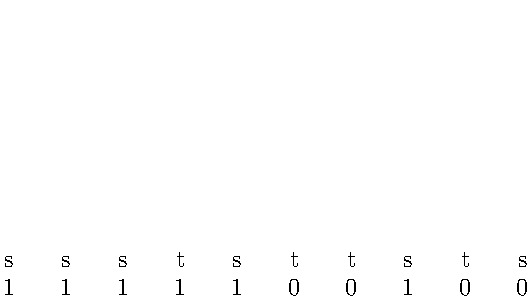
\includegraphics[width=0.7\textwidth]{anime/lightleaf_try2-1.pdf}}%
		\only<2>{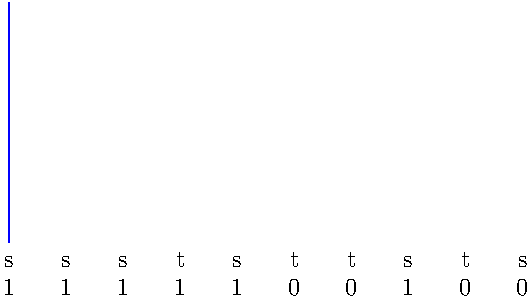
\includegraphics[width=0.7\textwidth]{anime/lightleaf_try2-2.pdf}}%
		\only<3>{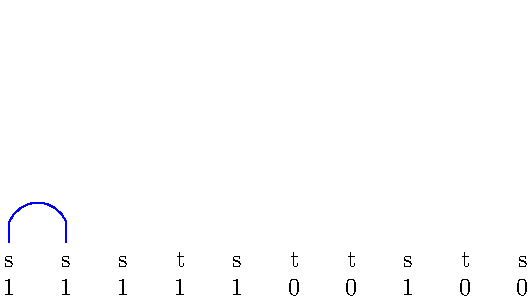
\includegraphics[width=0.7\textwidth]{anime/lightleaf_try2-3.pdf}}%
		\only<4>{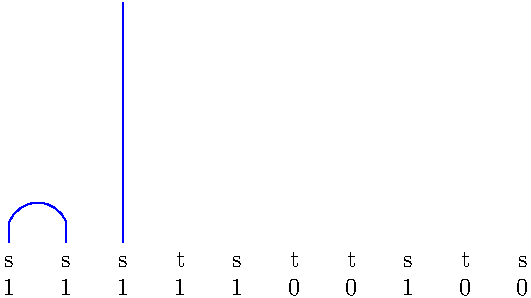
\includegraphics[width=0.7\textwidth]{anime/lightleaf_try2-4.pdf}}%
		\only<5>{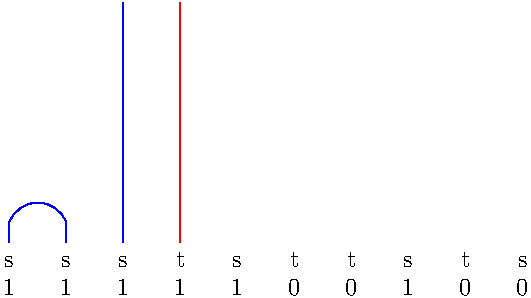
\includegraphics[width=0.7\textwidth]{anime/lightleaf_try2-5.pdf}}%
		\only<6>{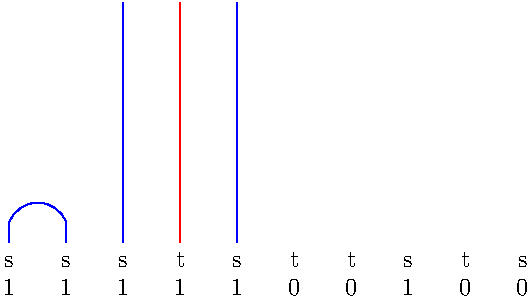
\includegraphics[width=0.7\textwidth]{anime/lightleaf_try2-6.pdf}}%
		\only<7>{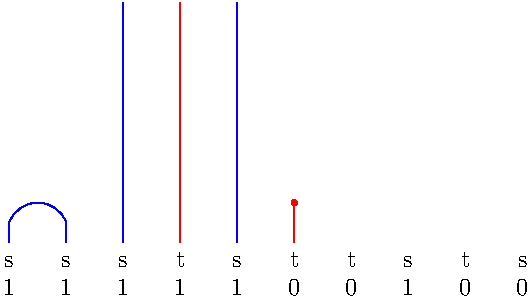
\includegraphics[width=0.7\textwidth]{anime/lightleaf_try2-7.pdf}}%
		\only<8>{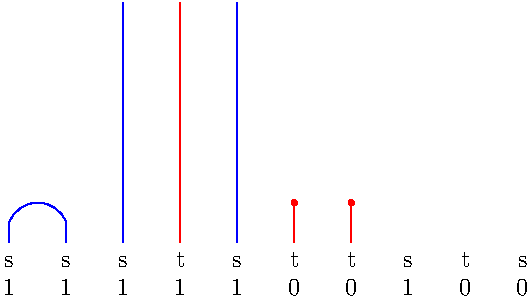
\includegraphics[width=0.7\textwidth]{anime/lightleaf_try2-8.pdf}}%
		\only<9>{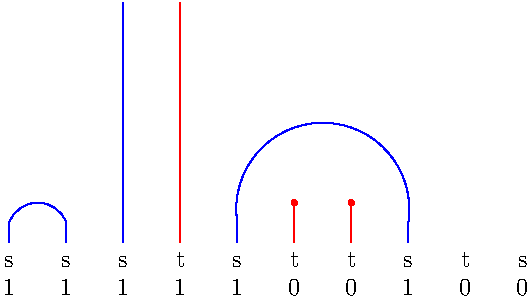
\includegraphics[width=0.7\textwidth]{anime/lightleaf_try2-9.pdf}}%
		\only<10>{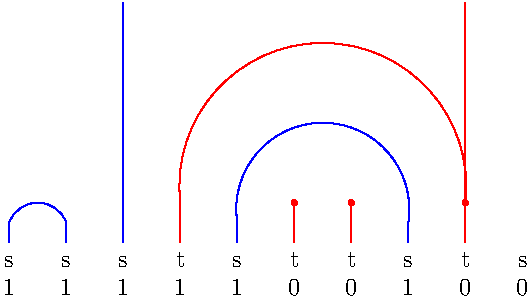
\includegraphics[width=0.7\textwidth]{anime/lightleaf_try2-10.pdf}}%
		\only<11>{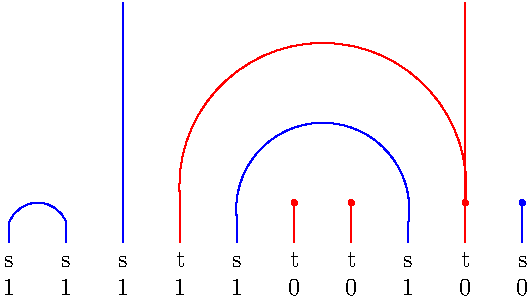
\includegraphics[width=0.7\textwidth]{anime/lightleaf_try2-11.pdf}}%
%		\only<1>{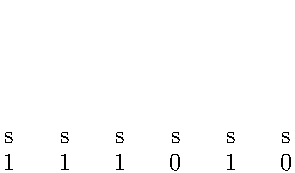
\includegraphics{anime/onecolor_example-1.pdf}}%
%		\only<2>{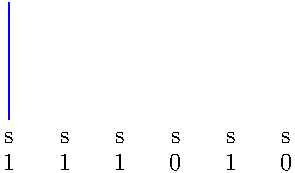
\includegraphics{anime/onecolor_example-2.pdf}}%
%		\only<3>{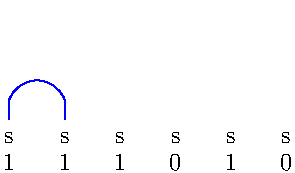
\includegraphics{anime/onecolor_example-3.pdf}}%
%		\only<4>{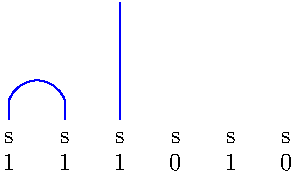
\includegraphics{anime/onecolor_example-4.pdf}}%
%		\only<5>{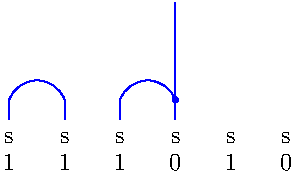
\includegraphics{anime/onecolor_example-5.pdf}}%
%		\only<6>{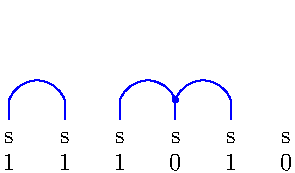
\includegraphics{anime/onecolor_example-6.pdf}}%
%		\only<7>{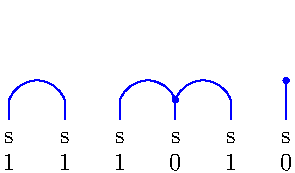
\includegraphics{anime/onecolor_example-7.pdf}}%
%		\only<8>{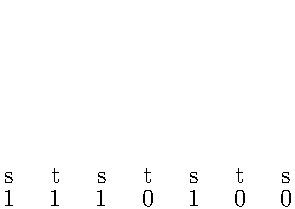
\includegraphics{anime/twocolor_example-1.pdf}}%
%		\only<9>{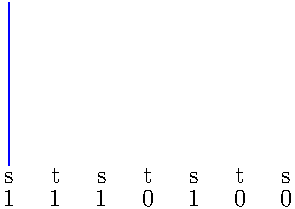
\includegraphics{anime/twocolor_example-2.pdf}}%
%		\only<10>{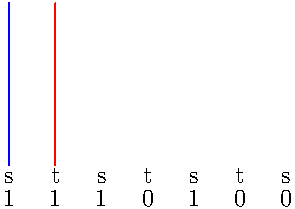
\includegraphics{anime/twocolor_example-3.pdf}}%
%		\only<11>{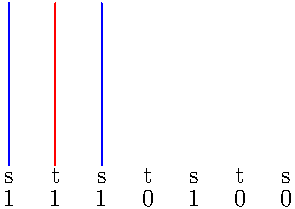
\includegraphics{anime/twocolor_example-4.pdf}}%
%		\only<12>{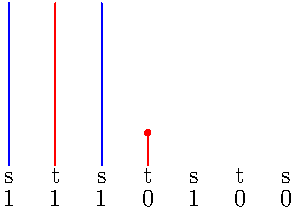
\includegraphics{anime/twocolor_example-5.pdf}}%
%		\only<13>{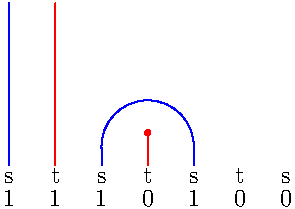
\includegraphics{anime/twocolor_example-6.pdf}}%
%		\only<14>{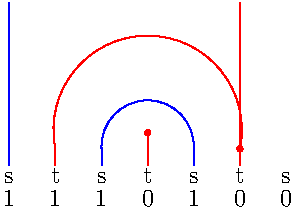
\includegraphics{anime/twocolor_example-7.pdf}}%
%		\only<15>{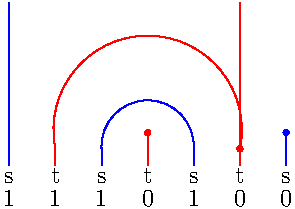
\includegraphics{anime/twocolor_example-8.pdf}}%
	\end{figure}
\end{frame}

\section{Problem Description}
\begin{frame}[fragile]
	\frametitle{Two Binary Strings}
	\begin{itemize}
		\ii Take a second binary string $\ul a$ (alongside with binary $\ul b$ and letters $\ul r$).
		\ii Associate polynomial in $\alpha_s$, $\alpha_t$, $x$, $y$, denoted $\boxed{\MM_{\ul r}(\ul a, \ul b)}$.
		\ii \alert{Goal}: compute this polynomial given $\ul a$, $\ul b$, $\ul r$.
	\end{itemize}
	\begin{figure}[ht]
		\centering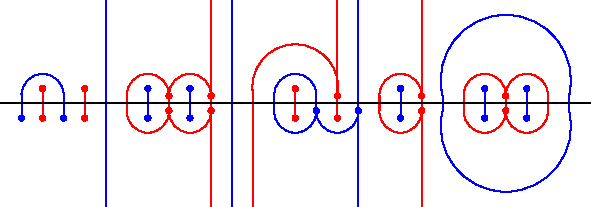
\includegraphics[height=3.4cm]{anime/compose_example-3.pdf}
	\end{figure}
\end{frame}

\begin{frame}
	\frametitle{What is this Polynomial?}
	\begin{enumerate}
	\ii (Barbells) When on the far left, $\barbell{barbell_blue} = \alpha_s$, while $\barbell{barbell_red} = \alpha_t$.
	\ii (Identity) When on the far right, $\barbell{wall_blue} = \barbell{wall_red} = 1$.
	\ii (Contraction) $\barbell{contract_left} = \barbell{contract_right} = \barbell{alpha_blue}$.
	\ii (Loops and Lower Terms) $\barbell{zero} = \barbell{lower_term} = 0$.
	\ii (Barbell-Forcing)
	$\barbell{alpha_blue} \barbell{barbell_blue} = 2 \barbell{break_blue} - \barbell{barbell_blue}\barbell{alpha_blue} $.  Furthermore, \\
	$\barbell{alpha_red}\barbell{barbell_blue} = -x\barbell{break_red} + \barbell{barbell_blue}\barbell{alpha_red} + x \barbell{barbell_red}\barbell{alpha_blue}$.
	% and $\barbell{alpha_blue}\barbell{barbell_red} = -y\barbell{break_blue} + \barbell{barbell_red}\barbell{alpha_blue} + y \barbell{barbell_blue}\barbell{alpha_red}$.
	\end{enumerate}
	For example, $\barbell{barbell_blue}\barbell{barbell_red}\barbell{barbell_blue}\barbell{alpha_blue} = \alpha_s^2\alpha_t$.
\end{frame}

\begin{frame}
	\frametitle{Recap}
	% Define block styles
	\tikzstyle{block} = [rectangle, draw, fill=blue!20, text width=6em, text centered, rounded corners, minimum height=4em]
	\tikzstyle{cloud} = [draw, ellipse,fill=red!20, node distance=3cm, text width=5em, text centered, minimum height=2em]
	\tikzstyle{line} = [draw, -latex']
	\scalebox{0.8}{
	\begin{tikzpicture}[node distance = 5cm, auto]
		% Place nodes
		\node [cloud] (Hecke) at (0,5) {Hecke algebra};
		\node [block] (Soergel) at (4,5) {Soergel bimodules};
		\node [block] (BS) at (8,5) {Category of Bott-Samelson bimodules};
		\node [block] (diag) at (8,2) {Diagrams};
		\node [cloud] (poly) at (8,0) {Polynomials};
		% Draw edges
		\path [line] (Hecke) -- (Soergel);
		\path [line] (Soergel) -- (BS);
		\path [line] (BS) -- node  {represented by} (diag);
		\path [line] (diag) -- node {correspond to} (poly);
	\end{tikzpicture}
	}
	\pause
	\hspace*{0.7\textwidth} $-x\alpha_s^2$

%	\begin{itemize}
%		\ii Complicated Hecke algebra described via Soergel bimodules.
%		\ii Soergel bimodules defined via Bott-Samelson bimodules.
%		\ii Maps between Bott-Samelson bimodules described by diagrams.
%		\ii Diagrams are translated into polynomials.
%	\end{itemize}
\end{frame}

\section{Results}
\begin{frame}
	\frametitle{Results}
	\begin{enumerate}
	\ii $\ul r = \underbrace{s\dots s}_{\text{length $n$}}$. \pause $\checkmark$
	\begin{theorem}
		There exists an explicit formula for $\MM_{s\dots s}(\ul a, \ul b)$ in terms of only the binary strings $\ul a$ and $\ul b$.
	\end{theorem}
	\pause
	\ii $\ul r = \underbrace{sts\dots}_{\text{length $n$}}$.
	\end{enumerate}
\end{frame}


\begin{frame}[fragile]
	\frametitle{Definitions}
%	\begin{definition}
%		\begin{itemize}
%			\ii \emph{Barbell}: acyclic component.
%			\ii \emph{Bubble}: bounded face.
%			\ii \emph{Caterpillar}: connected collection of bubbles.
%			\ii \emph{Fence}: dividing line.
%			\ii \emph{Pasture}: regions delimited by fences.
%		\end{itemize}
%	\end{definition}

	\begin{figure}[ht]
		\centering
		\begin{asy}
			size(10cm);
			real h = 0.7;
			int n = 16;

			picture one;
			draw(one, (0,0)--(0,h/2)..((0+2)/2.0,h*2)..(2,h/2)--(2,0), s);
			draw(one, (3,0)--(3,h/2)..((3+6)/2.0,h*3)..(6,h/2)--(6,0), s);
			draw(one, (9,0)--(9,h/2)..((9+11)/2.0,h*2)..(11,h/2)--(11,0), t);
			draw(one, (11,0)--(11,h/2)..((11+13)/2.0,h*2)..(13,h/2)--(13,0), t);
			draw(one, (13,0)--(13,h/2)..((13+15)/2.0,h*2)..(15,h/2)--(15,0), t);
			draw(one, (1,0)--(1,h), t);
			dot(one, (1,h), dot_t);
			draw(one, (4,0)--(4,h), t);
			dot(one, (4,h), dot_t);
			draw(one, (5,0)--(5,h), t);
			dot(one, (5,h), dot_t);
			draw(one, (10,0)--(10,h), s);
			dot(one, (10,h), dot_s);
			draw(one, (12,0)--(12,h), s);
			dot(one, (12,h), dot_s);
			draw(one, (14,0)--(14,h), s);
			dot(one, (14,h), dot_s);
			draw(one,(7,0)--(7,4*h), t);
			draw(one,(8,0)--(8,4*h), s);
			dot(one, (11, h/2), dot_t);
			dot(one, (13, h/2), dot_t);

			picture two;
			draw(two, (3,0)--(3,h/2)..((3+6)/2.0,h*3)..(6,h/2)--(6,0), s);
			draw(two, (9,0)--(9,h/2)..((9+11)/2.0,h*2)..(11,h/2)--(11,0), t);
			draw(two, (11,0)--(11,h/2)..((11+13)/2.0,h*2)..(13,h/2)--(13,0), t);
			draw(two, (13,0)--(13,h/2)..((13+15)/2.0,h*2)..(15,h/2)--(15,0), t);
			draw(two, (0,0)--(0,h), s);
			dot(two, (0,h), dot_s);
			draw(two, (1,0)--(1,h), t);
			dot(two, (1,h), dot_t);
			draw(two, (2,0)--(2,h), s);
			dot(two, (2,h), dot_s);
			draw(two, (4,0)--(4,h), t);
			dot(two, (4,h), dot_t);
			draw(two, (5,0)--(5,h), t);
			dot(two, (5,h), dot_t);
			draw(two, (10,0)--(10,h), s);
			dot(two, (10,h), dot_s);
			draw(two, (12,0)--(12,h), s);
			dot(two, (12,h), dot_s);
			draw(two, (14,0)--(14,h), s);
			dot(two, (14,h), dot_s);
			draw(two,(7,0)--(7,4*h), t);
			draw(two,(8,0)--(8,4*h), s);
			dot(two, (11, h/2), dot_t);
			dot(two, (13, h/2), dot_t);

			add(one); add(reflect((0,0),(1,0))*two);
			draw((-1,0)--(16,0));

			label("Pastures", (7.5,6*h));
			draw((7,5.5*h)--(4,4*h), EndArrow);
			draw((7.5,5.5*h)--(7.5,4*h), EndArrow);
			draw((8,5.5*h)--(11,4*h), EndArrow);
			label("Bubble", (4.5,-3*h), dir(-90));
			label("Fences", (7.5,-4*h), dir(-90));
			label("Barbells", (1, 4*h));
			draw((1,3.5*h)--(1,2.5*h), EndArrow);
			label("Caterpillar", (12,-2*h), dir(-90));
		\end{asy}
	\end{figure}
\end{frame}

\begin{frame}[fragile]
	\frametitle{Bubble Lemma}
	\begin{lemma}[Bubble Lemma]
		If $\ul r = stst\dots$, then
		every bubble contains either a single caterpillar or a single barbell.
	\end{lemma}
	\begin{figure}[ht]
		\centering
		\begin{asy}
		size(3cm);
		real h = 0.7;
		int n = 7;

		picture one;
		draw(one, (1,0)--(1,h/2)..((1+3)/2.0,h*2)..(3,h/2)--(3,0), t);
		draw(one, (3,0)--(3,h/2)..((3+5)/2.0,h*2)..(5,h/2)--(5,0), t);
		draw(one, (2,0)--(2,h), s);
		dot(one, (2,h), dot_s);
		draw(one, (4,0)--(4,h), s);
		dot(one, (4,h), dot_s);
		dot(one, (3, h/2), dot_t);

		picture two;
		draw(two, (1,0)--(1,h/2)..((1+3)/2.0,h*2)..(3,h/2)--(3,0), t);
		draw(two, (3,0)--(3,h/2)..((3+5)/2.0,h*2)..(5,h/2)--(5,0), t);
		draw(two, (2,0)--(2,h), s);
		dot(two, (2,h), dot_s);
		draw(two, (4,0)--(4,h), s);
		dot(two, (4,h), dot_s);
		dot(two, (3, h/2), dot_t);

		draw(CR((3,0),3), s);

		add(one); add(reflect((0,0),(1,0))*two);
		draw((-1,0)--(7,0));
		\end{asy}
		\caption{A bubble with a caterpillar inside it}
	\end{figure}
\end{frame}

\begin{frame}
	\frametitle{Other Lemmas}
	\begin{lemma}[Caterpillar Lemma]
		A blue caterpillar has associated polynomial $x^my^n\alpha_s$.
	\end{lemma}
	\pause
	\begin{lemma}[Pasture Lemma]
		Caterpillars appear only in the leftmost and rightmost pastures.
	\end{lemma}
\end{frame}

\begin{frame}
	\frametitle{Results}
	The lemmas allow us to get algebraic results when $\ul r = sts\dots$.
	\begin{theorem}
		If $\MM_{\ul r} (\ul a, \ul b)$ is nonzero with top $\ul w$, then it is
		\[
			x^{m}y^{n}\alpha_s^{u}\alpha_t^{v} \cdot
			\begin{cases}
				1 & \text{if $\ul w = \varnothing$ or $\ul w$ and $\ul r$ share a last char.} \\ 
				Q_{\ul w}  & \text{otherwise}
			\end{cases}
		\]
		for some nonnegative integers $m$, $n$, $u$, $v$.
		\label{thm:alt_struct}
	\end{theorem}
	Here $Q_{\ul w}$ is a \emph{quantum polynomial} with nice properties.
\end{frame}

%\begin{frame}[fragile]
%	\frametitle{Pasture Theorem}
%	\begin{theorem}[Pasture Theorem]
%		 If pastures are labelled $0, 1, \dots, N$ then:
%		\begin{itemize}
%			\ii Pastures $1$ through $N-1$ must contain caterpillars attached to fences.
%			\ii Pasture $N$ is either empty or contains a single caterpillar.
%		\end{itemize}
%	\end{theorem}
%	\begin{figure}[ht]
%		\centering
%		\begin{asy}
%			size(3cm);
%			real h = 0.7;
%			int n = 9;
%
%			picture one;
%			draw(one, (2,0)--(2,h/2)..((2+4)/2.0,h*2)..(4,h/2)--(4,0), s);
%			draw(one, (1,0)--(1,h/2)..((1+5)/2.0,h*4)..(5,h/2)--(5,0), t);
%			draw(one, (6,0)--(6,h/2)..((6+8)/2.0,h*2)..(8,h/2)--(8,0), s);
%			draw(one, (3,0)--(3,h), t);
%			dot(one, (3,h), dot_t);
%			draw(one, (7,0)--(7,h), t);
%			dot(one, (7,h), dot_t);
%			draw(one,(0,0)--(0,5*h), s);
%			draw(one,(5,0)--(5,5*h), t);
%			dot(one, (5, h/2), dot_t);
%
%			picture two;
%			draw(two, (2,0)--(2,h/2)..((2+4)/2.0,h*2)..(4,h/2)--(4,0), s);
%			draw(two, (1,0)--(1,h/2)..((1+5)/2.0,h*4)..(5,h/2)--(5,0), t);
%			draw(two, (6,0)--(6,h/2)..((6+8)/2.0,h*2)..(8,h/2)--(8,0), s);
%			draw(two, (3,0)--(3,h), t);
%			dot(two, (3,h), dot_t);
%			draw(two, (7,0)--(7,h), t);
%			dot(two, (7,h), dot_t);
%			draw(two,(0,0)--(0,5*h), s);
%			draw(two,(5,0)--(5,5*h), t);
%			dot(two, (5, h/2), dot_t);
%
%			add(one); add(reflect((0,0),(1,0))*two);
%			draw((-1,0)--(9,0));
%		\end{asy}
%		\caption{An attached caterpillar and a single caterpillar (each are singletons.)}
%	\end{figure}
%\end{frame}

\section{Closing}
\begin{frame}
	\frametitle{Acknowledgements}
	\begin{itemize}
		\ii Mr. Francisco Unda, MIT and Dr. Ben Elias, MIT
		\ii Antoni Rangachev, Northeastern University
		\ii Dr. Tanya Khovanova, Prof. Pavel Etingof, Dr. Vyacheslow Gerovitch; MIT Math Department
		\ii Sponsors: Ms. Alexa Margalith, The Leonetti/O'Connell Family Foundation; Mr. Arvind Parthasarathi, YarcData; Mr. Samuel Chen and Ms. Kathy Chang; Dr. Robert E. Curry; Mr. and Mrs. William Hellman; Mr. Rondal Hohauser; Ms. Chienlan Hsu-Hoffman; Mr. and Mrs. George Keiter
		\ii CEE and MIT, for hosting the RSI 2013.
	\end{itemize}
\end{frame}

\begin{frame}[fragile]
	\frametitle{Questions?}
	\begin{figure}[ht]
		\centering
		\begin{asy}
			size(10cm);
			real h = 0.7;
			int n = 27;

			picture one;
			draw(one, (0,0)--(0,h/2)..((0+2)/2.0,h*2)..(2,h/2)--(2,0), s);
			draw(one, (5,0)--(5,h/2)..((5+7)/2.0,h*2)..(7,h/2)--(7,0), t);
			draw(one, (7,0)--(7,h/2)..((7+9)/2.0,h*2)..(9,h/2)--(9,0), t);
			draw(one, (12,0)--(12,h/2)..((12+14)/2.0,h*2)..(14,h/2)--(14,0), s);
			draw(one, (11,0)--(11,h/2)..((11+15)/2.0,h*4)..(15,h/2)--(15,0), t);
			draw(one, (17,0)--(17,h/2)..((17+19)/2.0,h*2)..(19,h/2)--(19,0), t);
			draw(one, (21,0)--(21,h/2)..((21+23)/2.0,h*2)..(23,h/2)--(23,0), t);
			draw(one, (23,0)--(23,h/2)..((23+25)/2.0,h*2)..(25,h/2)--(25,0), t);
			draw(one, (20,0)--(20,h/2)..((20+26)/2.0,h*6)..(26,h/2)--(26,0), s);
			draw(one, (1,0)--(1,h), t);
			dot(one, (1,h), dot_t);
			draw(one, (3,0)--(3,h), t);
			dot(one, (3,h), dot_t);
			draw(one, (6,0)--(6,h), s);
			dot(one, (6,h), dot_s);
			draw(one, (8,0)--(8,h), s);
			dot(one, (8,h), dot_s);
			draw(one, (13,0)--(13,h), t);
			dot(one, (13,h), dot_t);
			draw(one, (18,0)--(18,h), s);
			dot(one, (18,h), dot_s);
			draw(one, (22,0)--(22,h), s);
			dot(one, (22,h), dot_s);
			draw(one, (24,0)--(24,h), s);
			dot(one, (24,h), dot_s);
			draw(one,(4,0)--(4,7*h), s);
			draw(one,(9,0)--(9,7*h), t);
			draw(one,(10,0)--(10,7*h), s);
			draw(one,(15,0)--(15,7*h), t);
			draw(one,(16,0)--(16,7*h), s);
			draw(one,(19,0)--(19,7*h), t);
			dot(one, (7, h/2), dot_t);
			dot(one, (23, h/2), dot_t);
			dot(one, (9, h/2), dot_t);
			dot(one, (15, h/2), dot_t);
			dot(one, (19, h/2), dot_t);

			picture two;
			draw(two, (5,0)--(5,h/2)..((5+7)/2.0,h*2)..(7,h/2)--(7,0), t);
			draw(two, (7,0)--(7,h/2)..((7+9)/2.0,h*2)..(9,h/2)--(9,0), t);
			draw(two, (12,0)--(12,h/2)..((12+14)/2.0,h*2)..(14,h/2)--(14,0), s);
			draw(two, (14,0)--(14,h/2)..((14+16)/2.0,h*2)..(16,h/2)--(16,0), s);
			draw(two, (17,0)--(17,h/2)..((17+19)/2.0,h*2)..(19,h/2)--(19,0), t);
			draw(two, (21,0)--(21,h/2)..((21+23)/2.0,h*2)..(23,h/2)--(23,0), t);
			draw(two, (23,0)--(23,h/2)..((23+25)/2.0,h*2)..(25,h/2)--(25,0), t);
			draw(two, (20,0)--(20,h/2)..((20+26)/2.0,h*6)..(26,h/2)--(26,0), s);
			draw(two, (0,0)--(0,h), s);
			dot(two, (0,h), dot_s);
			draw(two, (1,0)--(1,h), t);
			dot(two, (1,h), dot_t);
			draw(two, (2,0)--(2,h), s);
			dot(two, (2,h), dot_s);
			draw(two, (3,0)--(3,h), t);
			dot(two, (3,h), dot_t);
			draw(two, (6,0)--(6,h), s);
			dot(two, (6,h), dot_s);
			draw(two, (8,0)--(8,h), s);
			dot(two, (8,h), dot_s);
			draw(two, (13,0)--(13,h), t);
			dot(two, (13,h), dot_t);
			draw(two, (15,0)--(15,h), t);
			dot(two, (15,h), dot_t);
			draw(two, (18,0)--(18,h), s);
			dot(two, (18,h), dot_s);
			draw(two, (22,0)--(22,h), s);
			dot(two, (22,h), dot_s);
			draw(two, (24,0)--(24,h), s);
			dot(two, (24,h), dot_s);
			draw(two,(4,0)--(4,7*h), s);
			draw(two,(9,0)--(9,7*h), t);
			draw(two,(10,0)--(10,7*h), s);
			draw(two,(11,0)--(11,7*h), t);
			draw(two,(16,0)--(16,7*h), s);
			draw(two,(19,0)--(19,7*h), t);
			dot(two, (7, h/2), dot_t);
			dot(two, (14, h/2), dot_s);
			dot(two, (23, h/2), dot_t);
			dot(two, (9, h/2), dot_t);
			dot(two, (16, h/2), dot_s);
			dot(two, (19, h/2), dot_t);

			add(one); add(reflect((0,0),(1,0))*two);
			draw((-1,0)--(27,0));
		\end{asy}
		\caption{A large map with base $\AA_{27}$.}
		\label{fig:large_alt_example}
	\end{figure}
\end{frame}

\appendix
\section{Appendices}
\begin{frame}
	\frametitle{Bott-Samelson Bimodules}
	\begin{itemize}
		\ii $W = \left<s,t \mid s^2=t^2=1\right>$ is the infinite dihedral group.
		\ii $W$ acts on the Coxeter ring $R \defeq \RR[\alpha_s, \alpha_t]$ by $s(\alpha_s) = -\alpha_s$ and $s(\alpha_t) = \alpha_t + x\alpha_s$.
		\ii Define $R^s \defeq \left\{ r \in R \mid s(r) = r \right\}$ and $R^t$ similarly.
		\ii Bott-Samelson bimodules are \[ R \otimes_{R^{i_1}} R \otimes_{R^{i_2}} R \otimes_{R^{i_3}} \dots \otimes_{R^{i_n}} R, \]
where each $i_j$ is either $s$ or $t$.   We write elements of such a bimodule in the form $f_0 \mid f_1 \mid \dots \mid f_n$, where $f_i \in R$.
	\end{itemize}
\end{frame}

\begin{frame}
	\frametitle{Meaning of the Graphs}
	\emph{Demazure operator} $\partial_s: R \to R$ is $\partial_s(f) = \frac{f - s(f)}{\alpha_s}$.

	\begin{table}[ht]
		\[
		\begin{array}{rll}
			\text{Map} & \text{Modules} & \text{Description} \\[1em]
			\barbell{half_top} & R \stimes R \to R & 1 \mid 1 \mapsto 1 \\[1em]
			\barbell{half_bot} & R \to R \stimes R & 1 \mapsto \half \left( 1 \mid \alpha_s + \alpha_s \mid 1 \right) \\[1em]
			\barbell{tri_down} & R \stimes R \to R \stimes R \stimes R & 1 \mid 1 \mapsto 1 \mid 1 \mid 1 \\[1em]
			\barbell{tri_up} & R \stimes R \stimes R \to R \stimes R & 1 \mid g \mid 1 \mapsto \partial_s(g) \mid 1 \\[1em]
			\barbell{id} & R \stimes R \to R \stimes R & 1 \mid 1 \mapsto 1 \mid 1 \\[1em]
		\end{array}
		\]
		\caption{Describing the maps.}
	\end{table}
\end{frame}

\begin{frame}
	\frametitle{Quantum Numbers}
	\begin{definition}[Quantum Numbers]
		For each integer $n \ge 0$, define two polynomials $[n]_x, [n]_y \in \ZZ[x,y]$ recursively by $[0]_x = [0]_y = 0$, $[1]_x = [1]_y = 1$, $[2]_x = x$, $[2]_y = y$, and
	\[ [2]_x[n]_y = [n+1]_x - [n-1]_x \quad\text{and}\quad [2]_y[n]_x = [n+1]_y - [n-1]_y. \]
	\end{definition}

	\pause 

	\begin{definition}
		$Q_{\ul r} = [n+1]_x \alpha_s + [n]_y \alpha_t$ when $\ul r = stst\dots$ is length $n$.
	\end{definition}

	If $\ul r = ststs\dots$ has length $n+1$, then \[ \MM_{\ul r} ( \underbrace{11\dots11}_{\text{$n$ 1's}}0, \underbrace{11\dots11}_{\text{$n$ 1's}}0 ) = Q_{\ul r}. \]
\end{frame}

\begin{frame}
	\frametitle{One-Color Theorem}
	\begin{definition}
	For a binary string $\ul b$, let $\pi_1(\ul b)$ denote the number of $1$'s in $\ul b$.
	\end{definition}
	\begin{definition}
	For a binary string $\ul b$, define $\ul b^\ast$ by
	\[ \ul b^\ast [i] = \ul b[1] + \dots + \ul b[i] \pmod{2}. \]
	\end{definition}
	\pause
	\begin{theorem}
	If $\ul a, \ul b$ are compatible binary strings of length $n$,
	\[
		\MM_{sss\dots} \left( \ul a, \ul b \right)
		=
		\begin{cases}
			0 \text{ if } \exists 1 \le i \le n-1: \ul a^\ast[i] = \ul b^\ast[i] = 1 \\
			\alpha_s^{n - \pi_1(\ul a^\ast) - \pi_1(\ul b^\ast) + \ul a^\ast[n]} \text{ otherwise}.
		\end{cases}
	\]
	\end{theorem}
\end{frame}

\end{document}
